\section{开发环境和工具}
\subsection{开发环境}
软件采用 C++17，使用 Linux 文件系统、进程与网络接口，由 GNU Make 管理 CLI、服务端、测试程序及 GUI 构建目标。共享核心位于 \Code{include/} 与 \Code{src/}，前端入口位于 \Code{ui/} 和 \Code{app/}，服务端位于 \Code{server/}。核心不依赖 Qt，常用编译选项为 \Code{-Wall -Wextra -Wpedantic}。\E{E03}
\subsection{依赖库}
Qt 6 提供桌面界面，SQLite 保存服务端元数据。归档、压缩、加密及协议核心由项目实现。GoogleTest 用于测试组织；GNU tar、Zstd 命令行工具及 OpenSSL 等独立实现用于格式和算法对照。

\section{总体设计}
\subsection{系统结构设计}
\subsubsection{顶层系统结构}
系统分为表现层、共享核心、网络服务与持久化层。CLI 和 GUI 组织用户操作，共享核心完成扫描、过滤、编码、恢复和自动触发；网络客户端传输已生成的快照材料，服务端完成账户认证、文件存储及 SQLite 元数据管理。图形界面通过后台任务调用核心，避免长时间文件操作阻塞窗口。本地管理员工具负责服务实例、身份密钥和证书维护，管理员业务不作为公开网络操作提供。

\subsubsection{本地备份与还原子系统结构}
扫描器枚举目录条目，Filter 决定备份集合，打包层保存路径和元数据，压缩与加密层处理字节流。完整备份依次执行扫描、过滤、打包、可选压缩和可选加密，再封装为容器。恢复先识别并校验容器；加密归档通过认证后才解密，随后解压、预检路径、重建目录树并发布结果。定时与实时任务复用上述流程，增量备份模块根据已有快照和文件变化，决定创建完整备份、增量备份或跳过。

\subsubsection{远端子系统结构}
SecureChannel 负责握手和加密通信，RemoteArchiveClient 组织账户与快照请求，RemoteServer 处理连接，RemoteMetadataStore 管理数据库。连接先验证服务器身份，再进行注册、登录或会话恢复。固定 worker 池处理连接，数据库访问通过互斥锁和 busy timeout 协调。快照数据文件与数据库分开保存，服务端先保存快照文件，再按程序规定的顺序更新数据库记录。上传、下载均保存续传状态，重新连接后核对材料和位置再继续传输。\E{E03,E16}

\ReportLandscapeFigure{figures/pdf/07_component_system.pdf}{系统顶层构件图}{fig:component-system}
\ReportLandscapeFigure{figures/pdf/08_component_local.pdf}{本地备份与恢复子系统构件图}{fig:component-local}

\section{静态建模}
\subsection{系统对象模型}
对象模型按前端、本地核心、自动任务和网络服务划分。类图中的实心菱形表示组合，普通关联线表示非拥有引用。BackupEngine 持有 FileSystem；ScheduledBackupService 引用 ScheduleStore，调用方须保证存储对象的生命周期更长。多个本地控制器共享 GUI 写操作互斥控制对象（OperationGate），它记录当前操作持有者；获取与释放均在 GUI 主线程进行。远端服务为每条连接建立 SecureChannel 和 ConnectionContext，连接结束时清理上下文。
\begin{center}
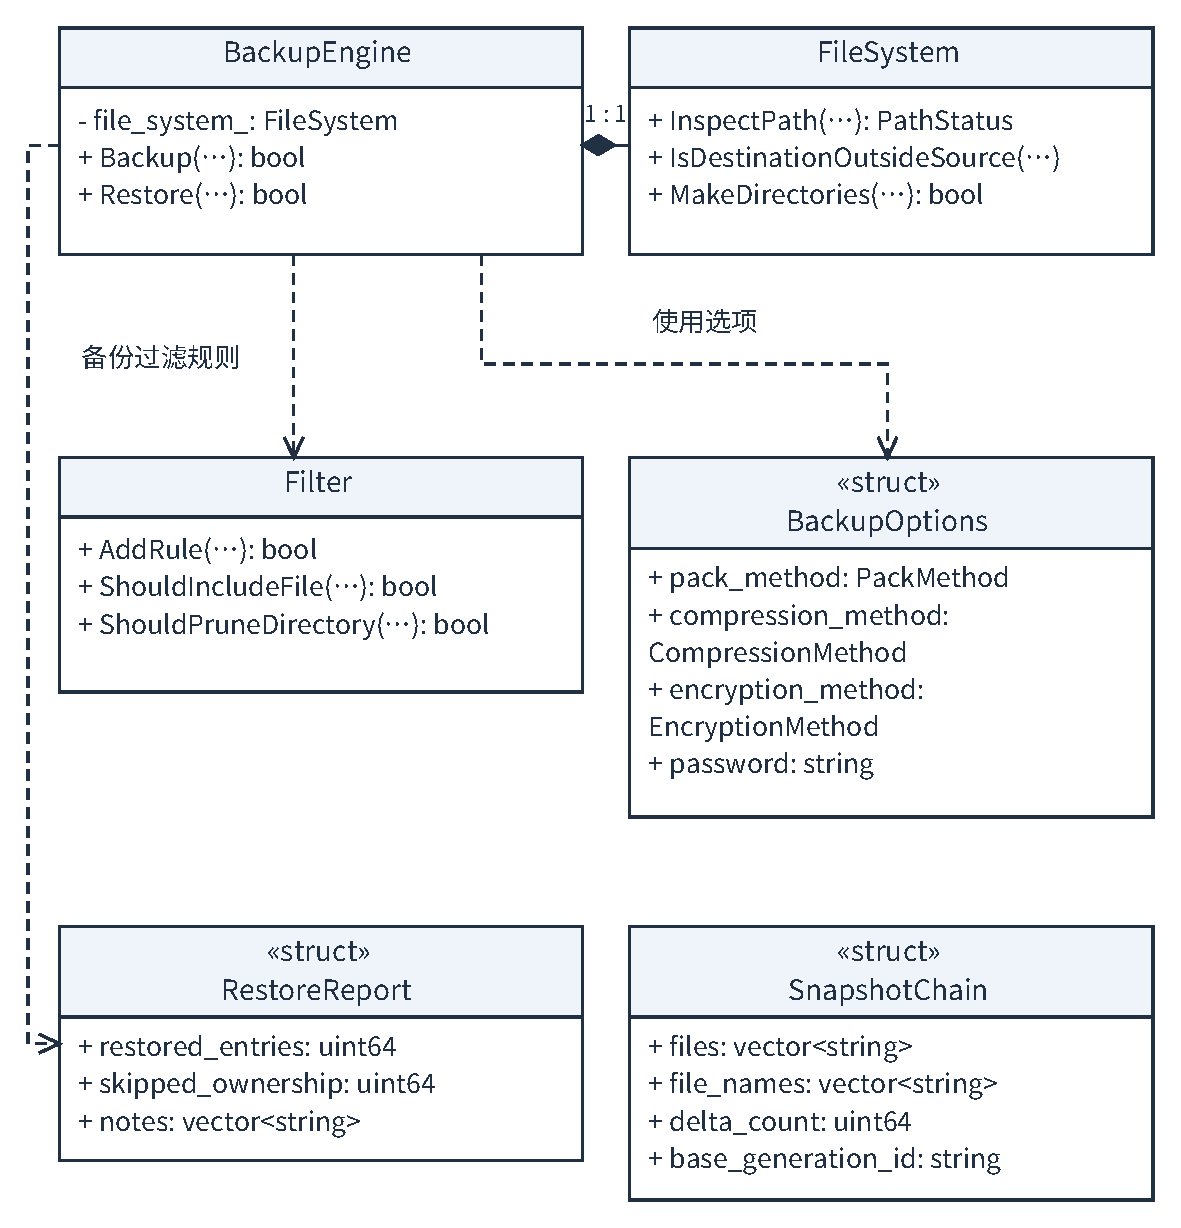
\includegraphics[width=.95\linewidth,height=.84\textheight,keepaspectratio]{figures/pdf/04_class_core.pdf}
\captionof{figure}{核心业务类图}\label{fig:class-core}
\end{center}

\subsection{类与数据结构描述}
主要类与结构体按前端、本地核心、自动任务及网络服务分组。表中列出关键属性、接口和对象关系；前端声明位于 \Code{ui/modern/}，其余声明位于 \Code{include/}，测试源码与脚本见 E13。
\begin{longtable}{@{}L{.22\linewidth}L{.34\linewidth}L{.38\linewidth}@{}}
\caption{前端控制器的类设计}\label{tab:classes-0}\\
\toprule 类或结构体 & 职责与关键属性 & 接口与对象关系\\\midrule\endfirsthead
\toprule 类或结构体 & 职责与关键属性 & 接口与对象关系\\\midrule\endhead
\bottomrule\endfoot

备份控制器\par\Code{BackupController} & 管理本地备份与恢复，将后台结果传递给界面。\par \nolinkurl{config\_manager\_}：ConfigManager；catalog\_：BackupCatalog；\nolinkurl{operation\_gate\_}：OperationGate*非拥有 & \nolinkurl{startBackupWithStrategy}、\nolinkurl{startManagedRestore}；Qt入口收集参数，成功 /\allowbreak 失败由核心结果回传；后台线程不直接更新 QML。\\\addlinespace[4pt]

定时任务控制器\par\Code{ScheduleController} & 计划配置、到期检查和删除观察。\par store\_：ScheduleStore；\nolinkurl{backup\_controller\_}为非拥有引用；共享 OperationGate & saveConfig、runNow、\nolinkurl{OnArchiveDeleted}；与备份控制器协调，不能在删除后重复获取同一 OperationGate。\\\addlinespace[4pt]

实时任务控制器\par\Code{RealtimeController} & 实时配置、监听和界面生命周期。\par watcher\_：\nolinkurl{InotifyWatcher}；debouncer\_：unique\_ptr<\allowbreak \nolinkurl{RealtimeDebouncer}>\allowbreak ；store\_：RealtimeStore & saveConfig、start、stop；任务执行进程关闭时不再产生新触发。\\\addlinespace[4pt]

写操作互斥控制\par\Code{OperationGate} & GUI主线程单持有者。\par owner\_：Kind，初始kNone & Acquire(Kind,QString*) $\to$\allowbreak bool；Release(Kind) $\to$\allowbreak void；busy() $\to$\allowbreak bool。获取非空且空闲才成功，释放必须匹配。\\\addlinespace[4pt]

\end{longtable}

\begin{longtable}{@{}L{.22\linewidth}L{.34\linewidth}L{.38\linewidth}@{}}
\caption{本地核心与数据结构的类设计}\label{tab:classes-1}\\
\toprule 类或结构体 & 职责与关键属性 & 接口与对象关系\\\midrule\endfirsthead
\toprule 类或结构体 & 职责与关键属性 & 接口与对象关系\\\midrule\endhead
\bottomrule\endfoot

应用配置管理器\par\Code{ConfigManager} & 应用配置文件编解码与原子替换。\par \nolinkurl{config\_file\_path\_}：std::string，由调用者显式给出 & Load(AppConfig*,string*) const $\to$\allowbreak \nolinkurl{ConfigLoadStatus}；Save(const AppConfig\&,string*) const $\to$\allowbreak bool；不处理仓库可用性。\\\addlinespace[4pt]

备份仓库目录管理器\par\Code{BackupCatalog} & 命名、解析、列表和依赖删除。\par 无持久实例成员；操作显式接收repository & List $\to$\allowbreak bool+\allowbreak vector<\allowbreak BackupRecord>\allowbreak ；\nolinkurl{BuildArchivePath} /\allowbreak Resolve /\allowbreak Delete /\allowbreak \nolinkurl{DeleteSnapshots} $\to$\allowbreak bool；归档头损坏时列出诊断。\\\addlinespace[4pt]

备份与恢复引擎\par\Code{BackupEngine} & 提供备份与恢复的统一接口，组织路径检查和处理流程。\par file\_system\_：FileSystem，按值组合 & Backup /\allowbreak Restore重载 $\to$\allowbreak bool；v2 options重载调用流水线，旧重载保留legacy语义。\\\addlinespace[4pt]

文件系统适配类\par\Code{FileSystem} & 路径检查和目录创建。\par 无持久实例成员；PathStatus枚举表示Missing /\allowbreak Directory /\allowbreak RegularFile /\allowbreak Other /\allowbreak Error & InspectPath(path,error) $\to$\allowbreak PathStatus；\nolinkurl{IsDestinationOutsideSource}、\nolinkurl{MakeDirectories} $\to$\allowbreak bool；系统错误通过诊断返回。\\\addlinespace[4pt]

文件过滤器\par\Code{Filter} & 解析过滤规则，决定目录剪枝及条目选择。\par rules\_：vector<\allowbreak Rule>\allowbreak ；Rule含action与vector<\allowbreak Clause>\allowbreak  & AddRule(action,text,error) $\to$\allowbreak bool，失败不变更；\nolinkurl{ShouldPruneDirectory} /\allowbreak \nolinkurl{ShouldIncludeFile} /\allowbreak \nolinkurl{ShouldSkipSpecialEntry} $\to$\allowbreak bool。\\\addlinespace[4pt]

备份选项结构体\par\Code{BackupOptions} & 保存本次备份的编码选项与口令。\par PackMethod pack\_method；\nolinkurl{CompressionMethod} \nolinkurl{compression\_method}；\nolinkurl{EncryptionMethod} \nolinkurl{encryption\_method}；string password & 默认MyPack /\allowbreak none /\allowbreak none；加密必须有口令，组合先由公共函数检查。\\\addlinespace[4pt]

恢复报告结构体\par\Code{RestoreReport} & 记录恢复结果、属主跳过数和诊断。\par uint64\_t \nolinkurl{restored\_entries}、\nolinkurl{skipped\_ownership}；vector<\allowbreak string>\allowbreak  notes & 由恢复调用逐步累积，不能将notes非空等同于整次失败。\\\addlinespace[4pt]

快照依赖链结构体\par\Code{SnapshotChain} & 保存从完整基线到目标快照的依赖顺序。\par vector<\allowbreak string>\allowbreak  files /\allowbreak file\_names；uint64\_t delta\_count；string \nolinkurl{target\_manifest\_digest} /\allowbreak \nolinkurl{base\_generation\_id} & 两个向量一一对应，base在前，target在后，解析自由函数填充。\\\addlinespace[4pt]

\end{longtable}

\begin{longtable}{@{}L{.22\linewidth}L{.34\linewidth}L{.38\linewidth}@{}}
\caption{自动备份与事件处理的类设计}\label{tab:classes-2}\\
\toprule 类或结构体 & 职责与关键属性 & 接口与对象关系\\\midrule\endfirsthead
\toprule 类或结构体 & 职责与关键属性 & 接口与对象关系\\\midrule\endhead
\bottomrule\endfoot

定时备份服务\par\Code{ScheduledBackupService} & 变化检测、任务执行与保留。\par string \nolinkurl{repository\_path\_}；ScheduleStore* store\_非拥有 & Evaluate /\allowbreak EvaluateNow $\to$\allowbreak bool+\allowbreak \nolinkurl{ScheduleEvaluationResult}；\nolinkurl{SetRepositoryPath} $\to$\allowbreak void；RunRetention $\to$\allowbreak bool，结果枚举需独立检查。\\\addlinespace[4pt]

计划存储类\par\Code{ScheduleStore} & 计划配置、状态、历史和manifest持久化。\par 文件路径字符串；与应用ConfigManager的schema分离 & Load /\allowbreak Save、LoadManifest /\allowbreak SaveManifest；分别读写计划文档与源清单；配置缺失和配置损坏采用不同状态。\\\addlinespace[4pt]

文件系统监听器\par\Code{InotifyWatcher} & Linux递归监听及事件收集。\par int fd\_；string root\_；vector<\allowbreak WatchTarget>\allowbreak  watches\_；索引映射 & Attach /\allowbreak Rebuild /\allowbreak Drain $\to$\allowbreak bool；Detach $\to$\allowbreak void。新监听fd建成才替换旧fd，根丢失 /\allowbreak overflow显式上报。\\\addlinespace[4pt]

实时事件去抖器\par\Code{RealtimeDebouncer} & 按静默窗口与最大等待时间合并事件。\par uint32\_t debounce\_ms\_ /\allowbreak max\_wait\_ms\_；bool dirty\_；int64\_t deadlines；uint64\_t event\_count\_ & NoteEvents /\allowbreak NoteResync $\to$\allowbreak void；Due $\to$\allowbreak bool；Consume $\to$\allowbreak \nolinkurl{RealtimeGeneration}；注入时间便于边界验证。\\\addlinespace[4pt]

\end{longtable}

\begin{longtable}{@{}L{.22\linewidth}L{.34\linewidth}L{.38\linewidth}@{}}
\caption{网络服务与存储的类设计}\label{tab:classes-3}\\
\toprule 类或结构体 & 职责与关键属性 & 接口与对象关系\\\midrule\endfirsthead
\toprule 类或结构体 & 职责与关键属性 & 接口与对象关系\\\midrule\endhead
\bottomrule\endfoot

远端归档客户端\par\Code{RemoteArchiveClient} & 组织远端请求并维护当前账户会话。\par int fd\_；bool \nolinkurl{authenticated\_}；string token\_；SecureChannel channel\_；\nolinkurl{RemoteEndpoint} endpoint\_ & Connect、Login、\nolinkurl{UploadSnapshotFile}、\nolinkurl{DownloadArchiveFile}、Delete $\to$\allowbreak bool；凭据不进入缓存或日志。\\\addlinespace[4pt]

安全传输通道\par\Code{SecureChannel} & BPSEC握手和认证加密记录。\par bool established\_；uint64\_t \nolinkurl{send\_sequence\_} /\allowbreak \nolinkurl{receive\_sequence\_}；双向密钥与会话材料 & \nolinkurl{HandshakeClient} /\allowbreak \nolinkurl{HandshakeServer}及证书变体、SendFrame /\allowbreak ReceiveFrame $\to$\allowbreak bool；失败不退明文，序号不能回绕。\\\addlinespace[4pt]

远端备份服务器\par\Code{RemoteServer} & 管理固定 worker 池及服务端启动、运行与停止。\par \nolinkurl{RemoteServerConfig} config\_；unique\_ptr<\allowbreak \nolinkurl{RemoteMetadataStore}>\allowbreak  store\_；unique\_ptr<\allowbreak \nolinkurl{RemoteMaintenance}>\allowbreak  maintenance\_；listener与workers\_集合 & Configure /\allowbreak Start /\allowbreak Run $\to$\allowbreak bool；RequestStop /\allowbreak Stop $\to$\allowbreak void；仅RequestStop允许与Run并发，认证原语是自由函数而非成员认证对象。\\\addlinespace[4pt]

远端元数据存储类\par\Code{RemoteMetadataStore} & SQLite元数据与链约束。\par sqlite3* database\_；string path\_；std::mutex mutex\_；不可复制 & Open /\allowbreak \nolinkurl{OpenExistingReadOnly} $\to$\allowbreak bool；\nolinkurl{InsertSnapshot} /\allowbreak Delete等 $\to$\allowbreak StoreResult；未打开时返回错误，应用层验证链。\\\addlinespace[4pt]

\end{longtable}


\subsubsection{核心操作的前后置条件}
BackupEngine 备份前检查源目录、输出位置和选项，成功后才发布所声明格式的归档。BackupCatalog 生成候选名称，实际写入通过排他创建避免重名覆盖；恢复与删除只接受仓库内合法的普通归档文件。依赖删除包含被删快照的后代，按后代优先执行，单个删除失败时停止并报告已处理项。

ConfigManager 区分配置已加载、首次缺失和内容错误。配置保存先写临时文件再替换旧文件；若替换后目录同步失败，返回失败时新内容可能已经可见，调用方应重新读取配置确认实际状态。Filter 的规则内子句取 AND，规则间取 OR，exclude 优先；规则解析失败不改变已生效规则。\E{E12}

自动任务将评估结果与执行结果分开记录。“立即执行”跳过到期判断，但源未变化时仍可跳过生成快照。保留策略同时维护可见还原点和其依赖祖先，对无法确认依赖或归属的对象保留并报告。监听器只收集事件，去抖器按静默窗口或最大等待合并事件；监听事件溢出或重同步时，由上层决定是否重新扫描源目录。

RemoteArchiveClient 持有通道和会话，业务失败返回诊断。RemoteServer 通过 RequestStop 向运行循环请求停止，运行线程统一回收连接和存储资源。RemoteMetadataStore 使用参数绑定执行 SQL，区分父链约束失败与内部错误；SecureChannel 维护双向密钥和报文序号，认证失败后终止会话。

\subsubsection{关键数据结构与自由函数模块}
BackupOptions 保存打包、压缩、加密选项和本次口令，RestoreOptions 提供恢复凭据。ArchiveEntry 表示路径、类型、权限、属主、时间、链接与设备信息；RestoreReport 保存恢复条目数、属主跳过数和诊断；SnapshotChain 保存从完整基线到目标快照的有序依赖。ConnectionContext 保存单条连接的认证身份、传输状态和文件描述符。

RunBackupPipeline、RunRestorePipeline、RunIncrementalBackup、ResolveSnapshotChain 和 RestoreSnapshotChain 等自由函数组织处理步骤。类图表示持有状态的对象及关系，构件图与顺序图表示函数模块之间的调用。

\subsection{其他静态建模方式}
数据库模型进一步描述账户、快照与注销记录的字段、键和索引；归档格式及增量身份结构见核心算法设计。

\section{动态建模}
\subsection{系统场景}
\subsubsection{场景一 手动完整备份}
控制器读取源目录、仓库、规则和编码选项，通过 OperationGate 获取操作权限后启动后台任务。共享核心扫描并过滤条目，经打包、压缩和加密后写入临时容器，成功同步后发布。完成通知返回 GUI 主线程，刷新列表并释放操作权限。任一步失败均向上层返回具体诊断。
\ReportLandscapeFigure{figures/report/pdf/09_sequence_backup_report.pdf}{GUI 手动完整备份顺序图：输入检查、任务启动与压缩}{fig:sequence-backup}
\ReportLandscapeFigureContinued[2]{figures/report/pdf/09_sequence_backup_report.pdf}{GUI 手动完整备份顺序图（续）：加密、写入与结果返回}{fig:sequence-backup-continued}
\ReportLandscapeFigure{figures/report/pdf/11_sequence_restore_chain_report.pdf}{受管增量链恢复顺序图：验证与完整基线恢复}{fig:sequence-restore-chain}
\ReportLandscapeFigureContinued[2]{figures/report/pdf/11_sequence_restore_chain_report.pdf}{受管增量链恢复顺序图（续）：增量处理与结果发布}{fig:sequence-restore-chain-continued}

\subsubsection{场景二 完整容器恢复}
系统检查容器头、长度与数据摘要；加密归档先验证 HMAC，再解密。解码后的打包流预检路径、重复项和父子关系，在恢复暂存目录（staging）中重建文件，最后应用元数据并发布结果。旧格式和裸 USTAR 使用各自的读取路径。

\subsubsection{场景三 增量链恢复}
系统先解析目标快照的完整依赖链，检查父身份、基线归属、环和链长。完整基线恢复到暂存目录，每个增量依次还原到增量恢复临时目录（overlay），按最深路径优先应用删除标记，再合并新增和修改项。任一步失败都中止整条链，全部成功后才发布目标。失败状态独立于诊断文本保存，调用方不接收错误文本时仍得到正确的失败返回值。\E{E10}

\subsubsection{场景四 远端增量备份}
客户端按配置验证证书或固定公钥摘要，完成握手后登录或恢复认证会话，核对远端基线并生成完整或增量快照。归档、manifest 和 identity 封装为 BPSNAP1 上传；服务端核对声明长度与 SHA-256，再发布数据文件并登记元数据。父子快照必须属于同一账户和备份链，代数连续且无分叉。上传中断时保留检查点，续传前重新核对已接收数据的摘要。

\subsubsection{场景五 远端快照下载与还原}
客户端查询本人快照及其依赖，复用已验证缓存或下载缺失材料。下载中断后使用保存的状态协商续传位置；完成后核对摘要和快照身份，解出 BPSNAP1 材料并复用本地链恢复。下载完成只表示文件已取回，用户选择恢复后才重建目录树。

\subsection{系统状态}
\subsubsection{服务端连接状态切换}
安全握手先于业务状态机。登录或 RESUME 成功后进入认证状态，开始传输时进入上传或下载状态，完成或中止后回到可继续请求的状态。非法顺序返回 InvalidState；断开连接时清理当前连接持有的临时文件及句柄。LOGOUT 清除本连接的认证状态，其他连接按各自令牌时效处理。

\subsubsection{GUI 写操作互斥控制（OperationGate）}
OperationGate 初始无持有者，空操作类型或已占用状态下获取失败；释放时须匹配当前持有者，OperationGuard 在退出作用域时负责释放。它协调手动备份、恢复、删除、仓库修改及定时、实时任务的配置和执行，共8类操作。远端控制器通过自身任务状态管理操作，进程级互斥由 ApplicationInstanceLock 实现。
\begin{center}
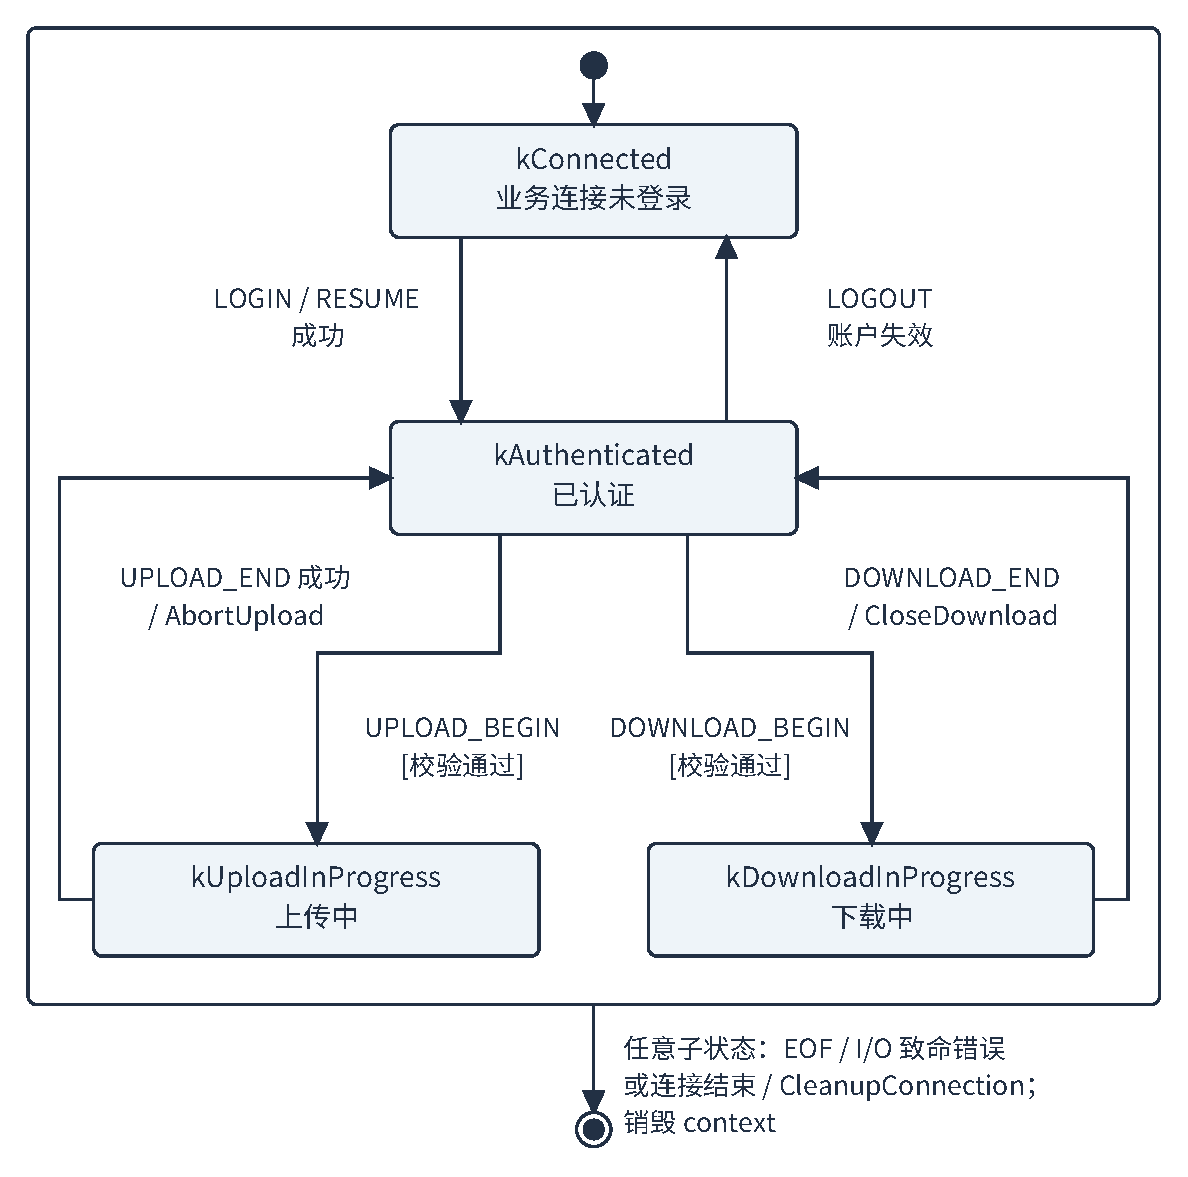
\includegraphics[width=.95\linewidth,height=.84\textheight,keepaspectratio]{figures/pdf/16_state_connection.pdf}
\captionof{figure}{远端连接状态转换图}\label{fig:state-connection}
\end{center}
\ReportLandscapeFigure{figures/pdf/17_state_operation_gate.pdf}{GUI 写操作互斥状态转换图}{fig:state-gate}

\section{数据库设计}
\subsection{引言}
SQLite 保存服务端账户、快照元数据和注销记录，归档字节保存在独立数据文件中。账户会话使用 HMAC 令牌，当前连接的认证状态保存在 ConnectionContext 中。
\subsection{数据库逻辑设计}
一个账户可拥有多个快照，增量快照关联一个父快照，同一父节点最多保留一个存活子节点。注销账户时删除其账户和快照元数据，并保存已注销用户 ID；用户 ID 显式分配且不复用，供旧令牌检查使用。用户名和凭据只保存在账户表，快照记录通过用户 ID 关联账户。
\subsection{数据库物理设计}
数据库使用 \Code{PRAGMA user_version=2} 标识结构版本。可写连接启用 foreign\_keys、WAL、synchronous=FULL 和 busy\_timeout；只读管理入口以 READONLY 和 query\_only 打开已有库。主键、用户名唯一约束及用户外键由 SQLite 检查，父快照同用户、同链、代数连续和无分叉由应用验证；父字段没有物理外键或唯一约束。
\subsection{基表设计}
\begin{longtable}{L{0.25\linewidth}L{0.13\linewidth}L{0.53\linewidth}}
\caption{users基表字段}\label{tab:db-users}\\\toprule 字段 & 类型 & 声明与业务含义\\\midrule\endfirsthead
\toprule 字段 & 类型 & 声明与业务含义\\\midrule\endhead
id & INTEGER & PRIMARY KEY； 用户 ID，整数主键\\
username & TEXT & NOT NULL；UNIQUE； 账户名，唯一且非空\\
password\_salt & BLOB & NOT NULL； 每用户随机salt，凭据派生参数\\
password\_hash & BLOB & NOT NULL； 派生口令校验值，不是明文口令\\
password\_iterations & INTEGER & NOT NULL； 口令派生迭代次数；业务层验证下限\\
created\_at & INTEGER & NOT NULL； 创建时间，整数时间戳\\
\bottomrule\end{longtable}

\begin{longtable}{L{0.25\linewidth}L{0.13\linewidth}L{0.53\linewidth}}
\caption{snapshots基表字段}\label{tab:db-snapshots}\\\toprule 字段 & 类型 & 声明与业务含义\\\midrule\endfirsthead
\toprule 字段 & 类型 & 声明与业务含义\\\midrule\endhead
id & TEXT & PRIMARY KEY； 快照 ID，文本主键\\
user\_id & INTEGER & NOT NULL； 所属账户，真实外键引用users(id)\\
display\_name & TEXT & NOT NULL； 展示名称，不作为服务端磁盘路径\\
size\_bytes & INTEGER & NOT NULL； 声明字节数；非负等语义由应用检查\\
sha256 & TEXT & NOT NULL； 归档/材料的SHA-256文本摘要\\
created\_at & INTEGER & NOT NULL； 创建时间，整数时间戳\\
storage\_name & TEXT & NOT NULL； 服务端生成的存储文件名\\
snapshot\_kind & INTEGER & NOT NULL；DEFAULT 0； 0完整/legacy独立，1增量；应用校验\\
parent\_id & TEXT & NOT NULL；DEFAULT ''； 无父为空串；没有数据库自外键\\
generation & INTEGER & NOT NULL；DEFAULT 0； 链代数，应用检查父+1和上限\\
lineage & TEXT & NOT NULL；DEFAULT ''； 应用层链归属标识；旧独立归档默认空串\\
\bottomrule\end{longtable}

\begin{longtable}{L{0.25\linewidth}L{0.13\linewidth}L{0.53\linewidth}}
\caption{deleted\_users基表字段}\label{tab:db-deleted_users}\\\toprule 字段 & 类型 & 声明与业务含义\\\midrule\endfirsthead
\toprule 字段 & 类型 & 声明与业务含义\\\midrule\endhead
id & INTEGER & PRIMARY KEY； 已注销用户 ID，整数主键\\
deleted\_at & INTEGER & NOT NULL； 注销时间，整数时间戳\\
\bottomrule\end{longtable}

\subsection{视图设计}
当前结构没有数据库视图。RemoteUserSummary 与 RemoteStorageOverview 是 SQL 聚合查询生成的结果结构体。\E{E09}
\subsection{索引设计}
\Code{snapshots_by_user(user_id, created_at, id)} 用于按用户列举及稳定排序，\Code{snapshots_by_parent(user_id, parent_id)} 用于后代查询和依赖删除。用户名唯一约束与快照主键还产生 SQLite 自动索引。

结构版本1升级到2时，在同一事务中追加链字段、依赖索引并更新版本号；失败回滚，重启可重试。旧记录按独立完整快照处理。

\ReportLandscapeFigure{figures/pdf/14_er_logical.pdf}{服务端数据库逻辑 E-R 图}{fig:er-logical}
\ReportLandscapeFigure{figures/pdf/15_er_physical.pdf}{服务端数据库物理 E-R 图}{fig:er-physical}

\section{核心算法与失败处理}
\enlargethispage{3\baselineskip}
\subsection{归档与编码}
MyPack、USTAR 和 Fast USTAR 均可用于完整及增量备份。后两者采用相同格式，区别在 I/O 策略。MyPack v2 全局头为32字节，条目头为64字节；外层 BKPCNT2 容器头为160字节。USTAR 的路径、链接名和八进制字段超出格式容量时拒绝写入，不截断数据。

当前压缩选项为不压缩、Canonical Huffman 和手写 Zstandard，旧 LZSS+Huffman 归档与任务保持兼容。Zstandard 按 RFC 8878 实现标准格式的一个子集：支持原始、RLE 和压缩块，原始、RLE 及显式权重 Huffman 字面量，预定义或 RLE 的 FSE 表，以及重复偏移和可选校验和。编码器按匹配和熵编码生成标准帧，无压缩收益时使用原始块。解码器拒绝字典、拼接帧、可跳过帧、动态或复用 FSE 表、复用 Huffman 表及 FSE 压缩的 Huffman 权重；窗口上限为8 MiB。\E{E16,E17}

编码流水线采用流式接口和私有临时文件控制缓冲规模；目录条目、manifest 和路径索引仍随文件数量增长。

\subsection{加密与服务器身份验证}
归档支持 AES-256-CTR-HMAC-SHA256 和 DES-CBC-HMAC-SHA256，DES 用于教学与兼容。随机 salt 与口令经 PBKDF2-HMAC-SHA256（200000轮）派生独立的加密密钥和 HMAC 密钥，IV 用于初始化加密过程。恢复先验证 HMAC，再解密，错误口令或认证失败时终止操作。

官方服务器的根公钥随客户端发行，服务器证书将服务器身份、公钥和有效期绑定到根签名。客户端验证可信根、证书有效期、预期 server\_id 及握手中的密钥证明后，才建立加密会话。BPSEC 使用 X25519 协商共享秘密，经 HKDF 派生双向密钥；报文认证和序号检查保护后续传输。错误身份、不可信根和未授权协议降级均拒绝。\E{E16,E17}

\subsection{文件级增量与自动触发}
manifest 记录文件内容摘要，用于区分新增、修改、删除和无变化。完整快照作为基线，增量保存变化条目及删除标记；未加密增量使用 BKPINC1，加密增量使用 BKPINC2 信封。BPIDENT3 将快照名、身份、manifest 摘要和格式绑定，加密场景使用密钥认证相关身份材料。恢复前验证完整依赖链，防止将不同基线或错误父节点拼接。BPSNAP1 用于远端传输归档及其两个副文件。\E{E10,E16}

定时和实时任务均支持完整、增量及加密组合。任务配置草稿保存并启用后生效，口令与普通配置分开管理：GUI 在当前会话解锁，CLI 可使用受权限保护的密码文件；加密任务缺少有效凭据时提示解锁或执行失败。实时任务合并文件事件，定时任务按周期检查；无变化时可跳过，任务状态与执行历史持久保存。

\subsection{文件发布、清理与现有限制}
临时文件通过排他创建建立归属依据，清理前核对文件身份；未确认由本次操作创建或身份无法验证的对象不递归删除。恢复在暂存目录中完成，全部必要步骤成功后再发布。单个目录项通过原子替换更新，归档、副文件、任务状态和数据库之间由业务流程协调，不构成一个跨文件事务。

现存文件系统限制包括：部分增量提取失败路径仍按路径名删除文件；目录身份检查与 unlinkat 之间存在 TOCTOU 竞争窗口；同 UID 进程可伪造所有权标记；已有空恢复目标可能在最终发布失败后消失。以上对应 FS-01 至 FS-04。属主和设备节点恢复还受 Linux 权限限制。\E{E04}
